%%%%%%%%%%%%%%%%%%%%%%%%%%%%%%%%%%%%%%%%%%%%%%%%%%%%%%%%%%%%%%%%%%%%%%%%%%%%%%%%
% Thesis / Project Report
% LaTeX Template
% Version 1.0 (08/04/14)
%
% Author:
% Darshit Shah
% https://github.com/darnir/BPHC-LaTeX-Report-Class
%
% This template is heavily based on the work of Steven Gunn and Sunil Patel
% Steven Gunn
% http://users.ecs.soton.ac.uk/srg/softwaretools/document/templates/
% and
% Sunil Patel
% http://www.sunilpatel.co.uk/thesis-template/
%
% License:
% CC BY-NC-SA 4.0 (http://creativecommons.org/licenses/by-nc-sa/4.0/)
%
% Note:
% Make sure to edit document variables in the Thesis.cls file
%
%%%%%%%%%%%%%%%%%%%%%%%%%%%%%%%%%%%%%%%%%%%%%%%%%%%%%%%%%%%%%%%%%%%%%%%%%%%%%%%%

%-------------------------------------------------------------------------------
%	PACKAGES AND OTHER DOCUMENT CONFIGURATIONS
%-------------------------------------------------------------------------------

\documentclass[11pt, a4paper, oneside]{Thesis} % Paper size, default font size
                                               % and one-sided paper

\graphicspath{{Pictures/}} % Specifies the directory where pictures are stored

\usepackage[square, numbers, comma, sort&compress]{natbib} % Use the natbib
                % reference package - read up on this to edit the reference
                % style; if you want text (e.g. Smith et al., 2012) for the
                % in-text references (instead of numbers), remove 'numbers'


\title{\ttitle} % Defines the thesis title - don't touch this

\begin{document}

\frontmatter % Use roman numbering style (i, ii...) for the pre-content pages

\setstretch{1.3} % Line spacing of 1.3

% Define page headers using FancyHdr package and set up for one-sided printing
\fancyhead{} % Clears all page headers and footers
\rhead{\thepage} % Sets the right side header to show the page number
\lhead{} % Clears the left side page header

\pagestyle{fancy} % Finally, use the "fancy" page style to implement the
                  %FancyHdr headers

% Input all the variables used in the document. Please fill out the
% variables.tex file with all your details.
%-------------------------------------------------------------------------------
%	DOCUMENT VARIABLES
%
%	Fill in the lines below to set the various variables for the document
%-------------------------------------------------------------------------------

%-------------------------------------------------------------------------------
% Your thesis title - this is used in the title and abstract
% Command: \ttitle
\thesistitle{OCR for Printed Telugu Documents}
%-------------------------------------------------------------------------------
% The document type: Thesis / report, etc.
% Command: \doctype
\documenttype{Mtech  Thesis}
%-------------------------------------------------------------------------------
% Your supervisor's name - this is used in the title page
% Command: \supname
\supervisor{Raghu \textsc{Akkili}}
%-------------------------------------------------------------------------------
% The supervisor's position - Used on Certificate
% Command: \suppos
\supervisorposition{Technology Consultant}
%-------------------------------------------------------------------------------
% Supervisor's institute
% Command: \supinst
\supervisorinstitute{Hp Enterprise}
%-------------------------------------------------------------------------------
% Your Co-Supervisor's name
% Command: \cosupname
%\cosupervisor{Dr. Barry \textsc{Drew}}
%-------------------------------------------------------------------------------
% Co-Supervisor's Position - Used on Certificate
% Command: \cosuppos
%\cosupervisorposition{Asst. Professor}
%-------------------------------------------------------------------------------
% Co-Supervisor's Institute
% Command: \cosupinst
%\cosupervisorinstitute{BITS-Pilani Hyderabad Campus}
%-------------------------------------------------------------------------------
% Your Examiner's name. Not currently used anywhere.
% Command: \examname
%\examiner{}
%-------------------------------------------------------------------------------
% Name of your degree
% Command: \degreename
\degree{Masters of Technology }
%-------------------------------------------------------------------------------
% The BITS Course Code for which this report is written
% COmmand: \ccode
%\coursecode{C421T}
%-------------------------------------------------------------------------------
% The name of the Course
% Command: \cname
\coursename{Mtech}
%-------------------------------------------------------------------------------
% Your name. Extend manually in case of multiple authors
% Command: \authornames
\authors{Krishna Swathi \textsc{Srikanta}}
%-------------------------------------------------------------------------------
% Your ID Number - used on the Title page and abstract
% Command: \idnum
\IDNumber{2018AB04062}
%-------------------------------------------------------------------------------
% Your address
% Command: \addressnames
\addresses{}
%-------------------------------------------------------------------------------
% Your subject area
% Command: \subjectname
\subject{}
%-------------------------------------------------------------------------------
% Keywords for this report.
% Command: \keywordnames
\keywords{}
%-------------------------------------------------------------------------------
% University details
% Command: \univname
\university{\texorpdfstring{\href{http://universe.bits-pilani.ac.in/} % URL
                {Birla Institute of Technology and Science}} % University name
                {Birla Institute of Technology and Science}}
%-------------------------------------------------------------------------------
% University details, in Capitals
% Command: \UNIVNAME
\UNIVERSITY{\texorpdfstring{\href{http://universe.bits-pilani.ac.in/} % URL
                {BIRLA INSTITUTE OF TECHNOLOGY AND SCIENCE}} % name in capitals
                {BIRLA INSTITUTE OF TECHNOLOGY AND SCIENCE}}
%-------------------------------------------------------------------------------
% Department Details
% Command: \deptname
\department{\texorpdfstring{\href{http://universe.bits-pilani.ac.in/hyderabad/mechanicalengineering/MechanicalEngineering} % Your department's URL
                {Mechanical Engineering}} % Your department's name
                {Mechanical Engineering}}
%-------------------------------------------------------------------------------
% Department details, in Capitals
% Command: \DEPTNAME
\DEPARTMENT{\texorpdfstring{\href{http://universe.bits-pilani.ac.in/hyderabad/mechanicalengineering/MechanicalEngineering} % Your department's URL
                {MECHANICAL ENGINEERING}} % Your department's name in capitals
                {MECHANICAL ENGINEERING}}
%-------------------------------------------------------------------------------
% Research Group Details
% Command: \groupname
\group{\texorpdfstring{\href{Research Group Web Site URL Here (include http://)}
                {Research Group Name}} % Your research group's name
                {Research Group Name}}
%-------------------------------------------------------------------------------
% Research Group Details, in Capitals
% Command: \GROUPNAME
\GROUP{\texorpdfstring{\href{Research Group Web Site URL Here (include http://)}
                {RESEARCH GROUP NAME (IN BLOCK CAPITALS)}}
                {RESEARCH GROUP NAME (IN BLOCK CAPITALS)}}
%-------------------------------------------------------------------------------
% Faculty details
% Command: \facname
\faculty{\texorpdfstring{\href{Faculty Web Site URL Here (include http://)}
                {Faculty Name}}
                {Faculty Name}}
%-------------------------------------------------------------------------------
% Faculty details, in Capitals
% Command: \FACNAME
\FACULTY{\texorpdfstring{\href{Faculty Web Site URL Here (include http://)}
                {FACULTY NAME (IN BLOCK CAPITALS)}}
                {FACULTY NAME (IN BLOCK CAPITALS)}}
%-------------------------------------------------------------------------------


%-------------------------------------------------------------------------------
%   NON-CONTENT PAGES
%-------------------------------------------------------------------------------
\maketitle
\Declaration
\Certificate
\Quotation{Thanks to my solid academic training, today I can write hundreds of
words on virtually any topic without possessing a shred of information, which is
how I got a good job in journalism.}{Dave Barry}

\begin{abstract}
Optical character recognition(OCR) is a well known process for converting text images to machine
editable text format. Applications of OCR include preserving old/historical documents in electronic
format, library cataloging, automatic reading for sorting of postal mail, bank cheques and forms as
base for many applications in Natural Language Processing(NLP). OCR is a difficult problem to
solve on real world data. In specific for Telugu language it is very difficult problem as single character
formed by a single vowel or consonant or it can be compound character consists of combination of
vowel and consonants.\\ 
\par
Conventional OCR approaches like Support Vector Machines(SVM) detect the characters by segmenting the image
til character level this gives poor results .In our approach we used Convolutional neural network and Long
short-term memory neural networks which takes directly  segmented word as input instead of character there
my improving the accuracy of OCR system.  

\end{abstract}

\begin{acknowledgements}
I Thank Raghu Akkili for his guidance \ldots
\end{acknowledgements}

%-------------------------------------------------------------------------------
%	LIST OF CONTENTS/FIGURES/TABLES PAGES
%-------------------------------------------------------------------------------

% The page style headers have been "empty" all this time, now use the "fancy"
% headers as defined before to bring them back
\pagestyle{fancy}

\lhead{\emph{Contents}} % Set the left side page header to "Contents"
\tableofcontents % Write out the Table of Contents

% Set the left side page header to "List of Figures"
\lhead{\emph{List of Figures}}
\listoffigures % Write out the List of Figures

 % Set the left side page header to "List of Tables"
\lhead{\emph{List of Tables}}
\listoftables % Write out the List of Tables

%-------------------------------------------------------------------------------
%	ABBREVIATIONS
%-------------------------------------------------------------------------------

\clearpage % Start a new page

 % Set the line spacing to 1.5, this makes the following tables easier to read
\setstretch{1.5}

\lhead{\emph{Abbreviations}} % Set the left side page header to "Abbreviations"
\listofsymbols{ll} % Include a list of Abbreviations (a table of two columns)
{
\textbf{CNN} & \textbf{C}onvolutional \textbf{N}eural \textbf{N}etwork \\
\textbf{LSTM} & \textbf{L}ong \textbf{S}hort \textbf{N}etwork \textbf{T}erm \textbf{M}emory\\
\textbf{CTC} & \textbf{C}onnectionist \textbf{T}emporal \textbf{C}lassification \\
%\textbf{Acronym} & \textbf{W}hat (it) \textbf{S}tands \textbf{F}or \\
}

%-------------------------------------------------------------------------------
%	PHYSICAL CONSTANTS/OTHER DEFINITIONS
%-------------------------------------------------------------------------------

% \clearpage % Start a new page

% % Set the left side page header to "Physical Constants"
% \lhead{\emph{Physical Constants}}

%  % Include a list of Physical Constants (a four column table)
% \listofconstants{lrcl}
% {
% Speed of Light & $c$ & $=$ & $2.997\ 924\ 58\times10^{8}\ \mbox{ms}^{-\mbox{s}}$ (exact)\\
% % Constant Name & Symbol & = & Constant Value (with units) \\
% }

%-------------------------------------------------------------------------------
%	SYMBOLS
%-------------------------------------------------------------------------------

\clearpage % Start a new page

\lhead{\emph{Glossary}} % Set the left side page header to "Symbols"

\listofnomenclature % List the nomenclature. (We use the glossaries package)

%-------------------------------------------------------------------------------
%	DEDICATION
%-------------------------------------------------------------------------------

\setstretch{1.3} % Return the line spacing back to 1.3

\pagestyle{empty} % Page style needs to be empty for this page

% Dedication text
\Dedicatory{I would like to dedicate this thesis to my University which taught
me how to deal with all sorts of bureaucracy while doing real work.}

\addtocontents{toc}{\vspace{2em}} % Add a gap in the Contents, for aesthetics

%-------------------------------------------------------------------------------
%	THESIS CONTENT - CHAPTERS
%-------------------------------------------------------------------------------

\mainmatter % Begin numeric (1,2,3...) page numbering

\pagestyle{fancy} % Return the page headers back to the "fancy" style

% Include the chapters of the thesis as separate files from the Chapters folder
% Uncomment the lines as you write the chapters

% Chapter 1

\chapter{Introduction} % Main chapter title

\label{Chapter1} % For referencing the chapter elsewhere, use \ref{Chapter1} 

\lhead{Chapter 1. \emph{Introduction}} % This is for the header on each page - perhaps a shortened title

%----------------------------------------------------------------------------------------

Optical character recognition(OCR) is a well known process for converting text images to machine
editable text format. During past few decades significant research work is reported in the OCR area.
In English there are many  OCR applications are available . Apart from English there
is significant amount of research have been done for languages like Chinese  and Japanese.
OCR gained so much research interest because of its potential applications in post offices, banks and
defense organizations. Other applications involve reading aid for the blind, preserving old/historical
documents in electronic format, library cataloging, automatic reading for sorting bank cheques and
applications in natural language processing(NLP) area.

OCR implemented for English language can not be applied for Indian languages as the single
character formation in the Indian language can be either simple character formed by single vowel
or consonant or compound character formed by combination of the vowel and consonants.

\textbf{Motivation:}The research in OCR area all other languages like English, Chinese and Japanese
are far a head compared to the research done in Indian languages. In particular the research done
in OCR for Telugu language is not significant. We want to develop an OCR which can mitigate the error 
due to segmentation improve the accuracy. We want to
digitalize the old/historical documents of Telugu language which are available in digital library of
India.

Rest of the report is organized as follows.In Chapter 2 we will describe the summary of the segmentation 
algorithm. In chapter 3 we will describe architecture of neural network we  experimented for
solving problem. In chapter 4 we will describe the conclusion and future work.
% Chapter 1

\chapter{Stages of OCR Process} % Main chapter title

\label{Chapter2} % For referencing the chapter elsewhere, use \ref{Chapter1} 

\lhead{Chapter 2. \emph{Introduction}} % This is for the header on each page - perhaps a shortened title

\section{Stages of OCR Process }
Optical Character Recognition is a complex process .To solve the problem of OCR we have chosen the following stages.
\begin{itemize}
  
  \item Preprossessing and Binarization.
  \item Line and Word Segmentation.
  \item Word recognition with CNN LSTM Neural Network.
  \item Data Preparation.
\end{itemize}


\section{Preprossessing and Binarization}
Preprocessing and Binarization is First stage of OCR process. In this stage we have corrected the skew and used ostu binarization algorithm to convert the RGB image into GrayScale by remove noise.

\section{Line and Word Segmentation}
This Stage of process segments the image into lines and further the line image are segmented into word images
Histogram projection method is used Horizontally to segment lines and Vertically to segment words from lines image
\begin{figure}[h]
\centering
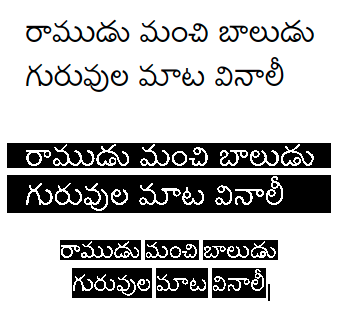
\includegraphics{Figures/image_segmentaion.png}
\caption{A Telugu Text Image Segmentation}
\end{figure}
% 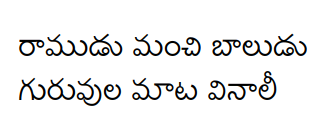
\includegraphics{Figures/my_tel_img.png} \\
% 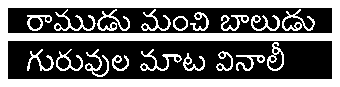
\includegraphics{Figures/merge_img.png}

\section{Word recognition with CNN LSTM Neural Network}
The Segmented Word Images are fed to Neural network which gives the text output .Since the Segmentaion is done at word level rather than character level accuracy is improved.

\section{Data Preparation}
Since there is Readily available OCR  data for Telugu language. words are taken from telugu corpus and used PIL tool to generate images from text.




%% Chapter 1

\chapter{Neural Network Architecture} % Main chapter title

\label{Chapter3} % For referencing the chapter elsewhere, use \ref{Chapter1} 

\lhead{Chapter 3. \emph{Introduction}} % This is for the header on each page - perhaps a shortened title

\section{Introduction} 

Neural Network is heart of OCR system ,the accuracy of OCR system heavily depends on accuracy of Neural
network . 

\section{Multi layer perceptron }

Multi layer perceptron is one of primitive neural network architecture . It contains artificial neurons
(which mimics the behaviour of human neuron) connected as layers as shown in \ref{fig:feed} The neural
network is trained by calculating loss and updating weights of perceptron  with back propagation algorithm 
most common activation function in percptron is Relu.


\begin{figure}[h]
\centering
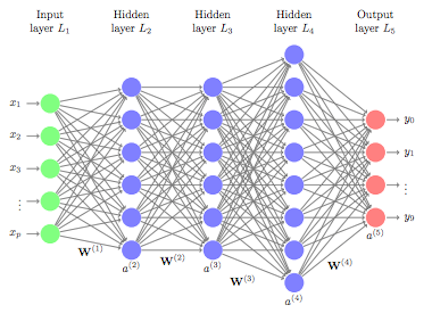
\includegraphics[width=15cm]{Figures/deep_nn.png}
\caption{Multilayer perceptron }
\label{fig:feed}
\end{figure}



\section{Convolutional neural network}
Convolutional Neural Networks  have a structure
similar to MLPs, but each layer is not fully-connected to the previous one. They
implement the notion of local receptors, via local connections and weight sharing. The
input is the two-dimensional image, and neurons in the hidden layers are organized in
two-dimensional maps, each looking for a single feature. Each neuron of a map is only
connected to a small neighborhood in the previous maps (or input image), with the
same connection weights as other neurons of the map . One may interpret
it as convolutions of the image with trainable filters.
\begin{figure}[h]
\centering
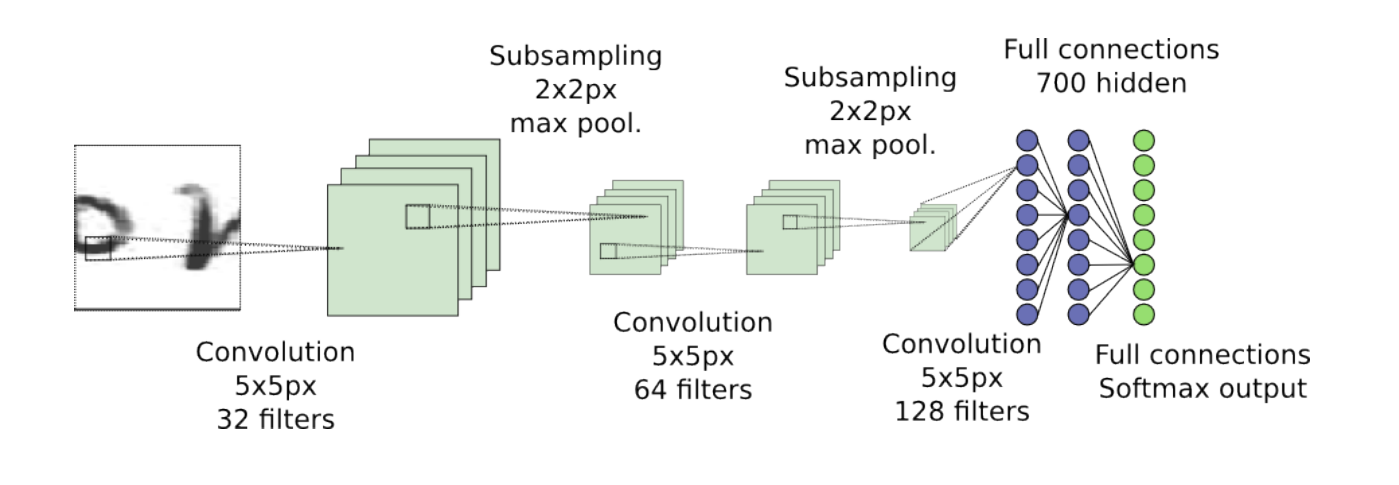
\includegraphics[width=15cm]{Figures/CNN.png}
\caption{ Convolutional neural network}
\label{fig:conv}
\end{figure}

The convolutional layers are often followed by subsampling layers, to limit the size of
the network and implement some invariance to distortions. The subsampling operation
may be a max-pooling or averaging over small neighborhoods. Usually, a few features
(or maps, or trainable filters) are extracted in lower layers, and increasingly more
features are extracted in upper layers, while the dimensions of the maps decrease (e.g.
in LeNet-5 .ConvNNs designed for classification can be easily extended to variable sized images,
hence producing sequences of predictions, thanks to the local connections and shared
weights

\section{Long short-term memory}
The output MLP and CNN just depend on input at present situation but some times we need to depend on the 
previous inputs also. RNN solves this type of problems . In Rnn the present output depends on present input
and also the previous inputs . but Classical RNN suffer from exploding and Vanishing gradient .LSTM Long Short Term Memory solves this issue with forgot gate. 
\begin{figure}[h]
\centering
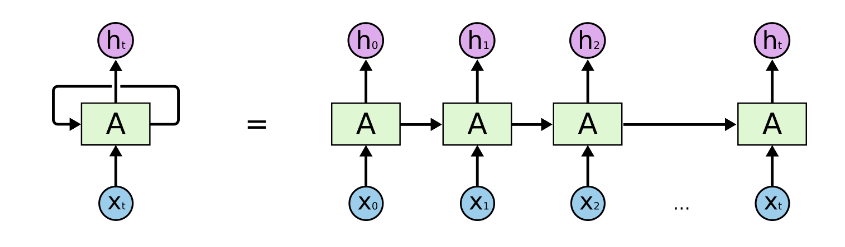
\includegraphics[width=15cm]{Figures/rnn.png}
\caption{ Reccurent neural network}
\label{fig:rnn}
\end{figure}

\begin{figure}[h]
\centering
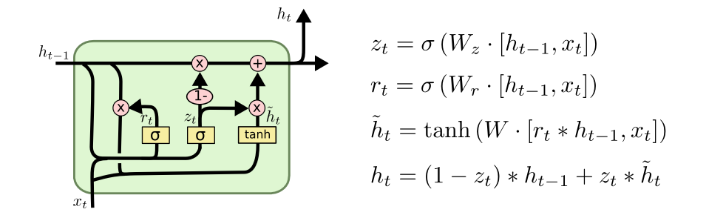
\includegraphics[width=15cm]{Figures/lstm.png}
\caption{ LSTMnetwork}
\label{fig:lstm}
\end{figure}

\section{Connectionist Temporal Classification}
\begin{figure}[h]
\centering
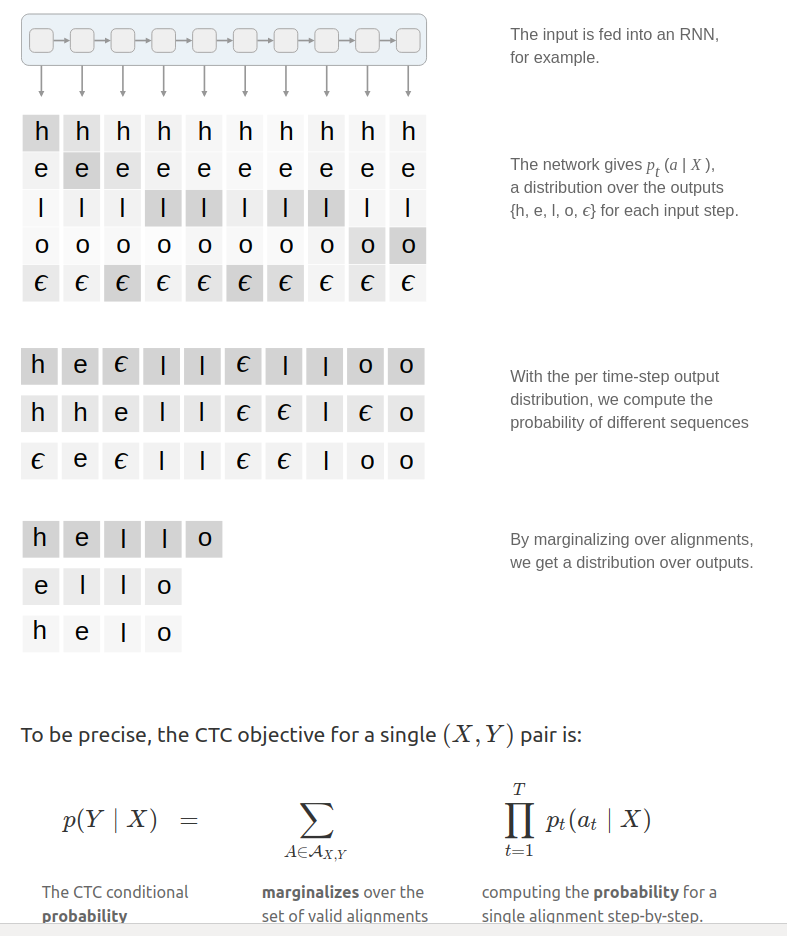
\includegraphics[width=15cm]{Figures/ctc.png}
\caption{ CTC LOSS}
\label{fig:CTC}
\end{figure}


\section{Architecture of OCR Neural Network}

CNN are good at objection recognition and LSTM are good at seq data prediction . To predict the image with
out segmentation we have to feed the image as sequence of pixels.ie we have to predict it with LSTM but LSTM
are hard to train and can't predict well on long sequence. So we have to extract important features from 
image to train a LSTM . CNN comes in handy for extracting  features from given image there by reduces the 
dimension of input. 


The architecture is shown in figure \ref{fig:arch}.The Neural network consist It consists of 7
convolutional layers these layers help to extract the important features to feed to LSTM. 7 CNN layers were
chosen so that the Neural Network will not over fit on large dataset .Batch normalization and drop out
techniques were used to improve the generalization of the network. Finally the Bidirectional LSTM recognizes
the word .Since LSTM are hard to train for long duration the number of CNN layers were kept more to increase
the recognition capacity of the network.CTC loss is used to calculation the loss and train the network
.Language model corrects the CTC decoded output.

\begin{figure}[h]
\centering
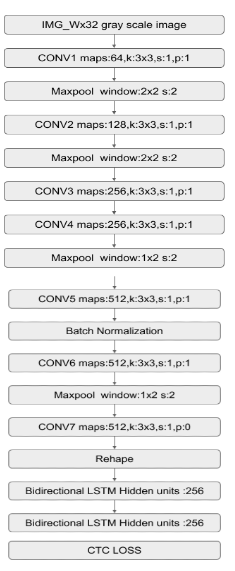
\includegraphics{Figures/arch.png}
\caption{Neural Network Architecture}
\label{fig:arch}
\end{figure}

%\input{Chapters/Chapter4}
%\input{Chapters/Chapter5}
%\input{Chapters/Chapter6}
%\input{Chapters/Chapter7}

%-------------------------------------------------------------------------------
%	THESIS CONTENT - APPENDICES
%-------------------------------------------------------------------------------

\addtocontents{toc}{\vspace{2em}} % Add a gap in the Contents, for aesthetics

\appendix % Cue to tell LaTeX that the following 'chapters' are Appendices

% Include the appendices of the thesis as separate files from the Appendices
% folder
% Uncomment the lines as you write the Appendices

% Appendix A

\chapter{Appendix Title Here} % Main appendix title

\label{AppendixA} % For referencing this appendix elsewhere, use \ref{AppendixA}

\lhead{Appendix A. \emph{Appendix Title Here}} % This is for the header on each page - perhaps a shortened title

Write your Appendix content here.
%\input{Appendices/AppendixB}
%\input{Appendices/AppendixC}

\addtocontents{toc}{\vspace{2em}} % Add a gap in the Contents, for aesthetics

\backmatter

%-------------------------------------------------------------------------------
%	BIBLIOGRAPHY
%-------------------------------------------------------------------------------

\label{Bibliography}

\lhead{\emph{Bibliography}} % Change the page header to say "Bibliography"

% Use the "unsrtnat" BibTeX style for formatting the Bibliography
\bibliographystyle{ieeetr}

% The references (bibliography) information are stored in the file named
% "Bibliography.bib"
\bibliography{Bibliography}

\end{document}
